\section{Project Summary}

The proposed sculpture is a grid of metal plates installed on the wall.
Each plate is controlled by a motor, giving it one degree of freedom of motion vertically.
The default motion for the plates is a wave-like pattern, as demonstrated in the attached video.
When a motion sensor is tripped, the plates switch behaviors to collectively move to, and wait at, the top or bottom of the grid.
After X minutes, the plates resume their wave-like pattern. 
The motion sensor is then disabled for Y minutes\footnote{The value for X and Y remain to be experimentally determined during beta testing of installation.}.

\begin{figure}[h!]
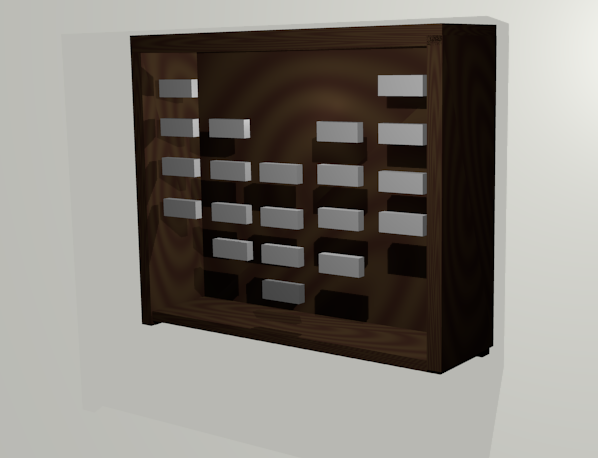
\includegraphics[width=0.48\textwidth]{../Test.png}
\label{fig:render}
\caption{A very rough render of the proposed physical installation because 3D modeling is hard.}
\end{figure}

The proposed sculpture aims to embody the particle-wave duality phenomena and the quantum state collapse under observation.
By providing a large-scale physical manifestation of core concepts in quantum theory, I hope to give visitors to YQI an immediate intuition to the work happening at the institute.



The code to control the plates is itself an artistic creation, and will be posted along with the explanation of the sculpture.
As an example, we list code here describing the transitions between quantum states.

\begin{figure}
\begin{lstlisting}
changeQState (observed,q,plates) = if
  | observed && q==Classic -> ReQuantize
  | observed && q==Quantum -> Classic
  | observed && q==ReQuantize -> Classic
  | q==ReQuantize -> 
      if inOrigPos plates 
      then Quantum else ReQuantize
  | otherwise -> q

\end{lstlisting}
\label{fig:code}
\caption{Code as art}
\end{figure}


If accepted, and with the approval of the board, I would like to dedicate this installation to Paul Hudak.
As a founder of FARM (in addition to Haskell and FRP), using Haskell in a public work of art in a quantum physics lab seems to capture a small part of the vision Paul had for the boundless possibilities at the intersection of logic and imagination.

\subsection{Schedule}

% hm this is pretty labor intensive. I think I need to simplify the build
% use graphviz
\begin{enumerate}
\item Manufacture one test set of plates on wires (Nov 20)
item Manufacture test motor with winding extension
\item Test build one column with manually controlled motors (Nov 25)
\item Arduino controlling single motor connected to plate (Dec 1)
\item Arduino controlling motors for one column (Dec 5)
\item Arduino controlling 20 motors (Dec 15)
\item Arduino taking input from motion sensor (Feb18)
\item Begin installation in space (Feb 17)
\item Finish installation (Feb 28)
\end{enumerate}

\subsection{Budget}

Because the work for this project will be funded under the grant, I cannot accept payment for the art.
I will only request funding for materials.


\begin{table}[h!]
\centering
\caption{Itemized Budget for materials}
\label{table:results}
\vspace{0.4em}
\begin{tabular}{|l|r|r|r|}
\hline
\multicolumn{1}{|c|}{\multirow{2}{*}{\textsc{Item}}} 
  & \multicolumn{1}{c|}{\multirow{2}{*}{\textsc{Cost} \scriptsize{(\$)} \textsc{/ Unit}}}
  & \multicolumn{1}{c|}{\multirow{2}{*}{\textsc{Quantity}}}
  & \multicolumn{1}{c|}{\multirow{2}{*}{\textsc{Total Cost} \scriptsize{(\$)}}} \\ 
& \multicolumn{1}{c|}{\textsc{}} & \multicolumn{1}{c|}{\textsc{}} & \\
\hline \hline
\textbf{Grid} & & & \\[-0.2em]
\quad Plates & 15.00 & 20 & 3.00  \\
\quad 5lb Fishing Line & 3.00 & 10ft & 3.00  \\
\hline 
\textbf{Frame} & & & \\[-0.2em]
\quad Museum Glass  & 2.083   & 1 & 7  \\    
\quad Vancouver Maple  & 2.032   & 1 & 6  \\
\hline 
\textbf{Electronics} & & & \\[-0.2em]
\quad Arduino   & 0.036   & 1 & 0  \\ % escalator0
\quad Motion sensor & 0.041   & 1 & 3  \\ % escalator1
\quad 5lb Stepper Motor & 11.50 & 20 & 2  \\
\hline 
\end{tabular}
\vspace{-1.5em}
\ 
\end{table}

\subsection{Extensions}

This project also has the potential to be extended to capture the idea of quantum intangelment.
I hope to install this same sculpture at Yale NUS in Singapore, with a small addition.
The Yale New Haven sculpture will be connected to the Yale NUS sculpture over the internet.
Whenever the motion sensor is triggered for one sculpture, thereby collapsing the state to a 0 or 1, the paired sclupture will also collapse to the complement state.


